You are given the following data situation:
\begin{knitrout}
\definecolor{shadecolor}{rgb}{0.969, 0.969, 0.969}\color{fgcolor}\begin{kframe}
\begin{alltt}
\hlkwd{library}\hlstd{(ggplot2)}
\hlkwd{library}\hlstd{(mlr3)}

\hlcom{# generate 200 nonlinear separable binary observations}
\hlkwd{set.seed}\hlstd{(}\hlnum{123}\hlstd{)}
\hlstd{moon_data} \hlkwb{=} \hlkwd{tgen}\hlstd{(}\hlstr{"moons"}\hlstd{)}\hlopt{$}\hlkwd{generate}\hlstd{(}\hlnum{200}\hlstd{)}\hlopt{$}\hlkwd{data}\hlstd{()}

\hlstd{moon_data}\hlopt{$}\hlstd{y} \hlkwb{=} \hlkwd{ifelse}\hlstd{(moon_data}\hlopt{$}\hlstd{y} \hlopt{==} \hlstr{"A"}\hlstd{,} \hlnum{1}\hlstd{,} \hlopt{-}\hlnum{1}\hlstd{)}
\hlstd{moon_data}\hlopt{$}\hlstd{y_dec} \hlkwb{=} \hlkwd{as.factor}\hlstd{(moon_data}\hlopt{$}\hlstd{y)}

\hlkwd{ggplot}\hlstd{(moon_data,} \hlkwd{aes}\hlstd{(}\hlkwc{x}\hlstd{=x1,} \hlkwc{y}\hlstd{=x2))} \hlopt{+}
  \hlkwd{geom_point}\hlstd{(}\hlkwd{aes}\hlstd{(}\hlkwc{color}\hlstd{=y_dec))} \hlopt{+}
  \hlkwd{xlab}\hlstd{(}\hlkwd{expression}\hlstd{(x[}\hlnum{1}\hlstd{]))} \hlopt{+}
  \hlkwd{ylab}\hlstd{(}\hlkwd{expression}\hlstd{(x[}\hlnum{2}\hlstd{]))} \hlopt{+}
  \hlkwd{labs}\hlstd{(}\hlkwc{color}\hlstd{=}\hlkwd{expression}\hlstd{(y))}
\end{alltt}
\end{kframe}
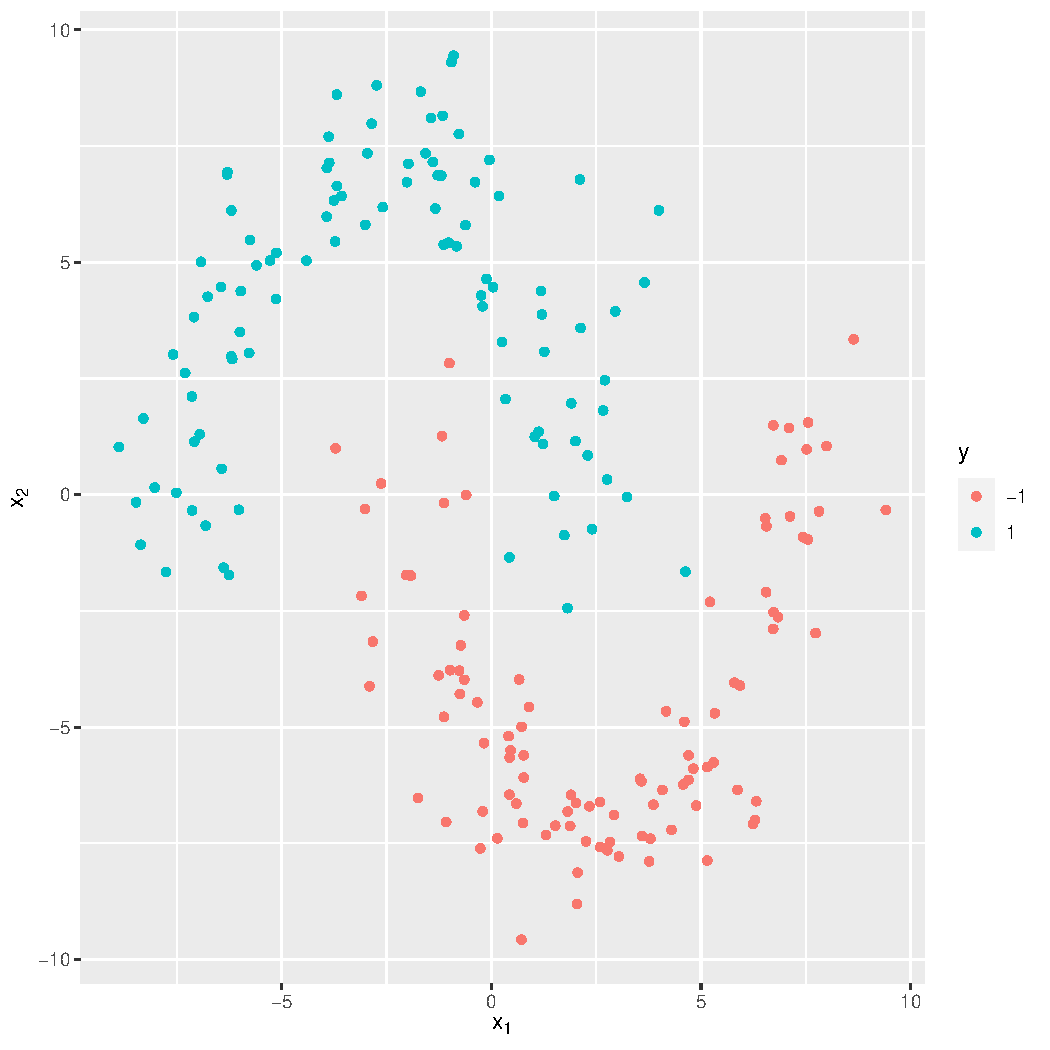
\includegraphics[width=0.5\linewidth]{figure/nonlindata-plot-1} 
\end{knitrout}
\\ 
We can extend the linear SVM to a nonlinear SVM by transforming the features via a nonlinear transformation $\phi:\R^d \rightarrow \R^l.$ With this, the primal form with soft constraints becomes
$$\min_{\bm{\theta}, \theta_0, \bm{\zeta}} 0.5\Vert \bm{\theta} \Vert^2 + C\sum^n_{i=1}\zeta^{(i)}$$ \\
s.t. $$y^{(i)}(\langle\bm{\theta}, \phi(\mathbf{x}^{(i)})\rangle + \theta_0) \leq 1 - \zeta^{(i)}\quad\forall i \in\{1,\dots,n\}$$ \\
and  
$$\zeta^{(i)} \geq 0\quad \forall i \in\{1,\dots,n\}.$$

\begin{enumerate}
\item Write down the general Lagrangian function of the nonlinear SVM
\item Solve the primal nonlinear SVM for $C=1$ and third order polynomial transformation (without intercept) $\phi(\mathbf{x}) = (x_1, x_2, x_1^2, x_2^2, x_1^3, x_2^3, x_1x_2, x_1^2x_2, x_1x_2^2)^\top$ with $\texttt{cvxr}$ in $\texttt{R}.$ \\
\textit{Hint:} Examples how quadratic problems can be solved with $\texttt{cvxr}$ can be found \href{http://www.di.fc.ul.pt/~jpn/r/optimization/CVXR.html#quadratic-programming}{here}.
\item State the KKT conditions of the general nonlinear SVM
\item Derive the dual form of the nonlinear SVM. State an advantage of the dual form over the primal form. \\
\textit{Hint:} Use the KKT conditions to transform the primal form
\item Solve the dual form of b) with $\texttt{cvxr}$ in $\texttt{R}.$ \\
\textit{Hint 1}: For a polynomial transformation $\phi$ of order $l$ (without intercept) it holds that there exists a invertible diagonal matrix $\mathbf{D} \in \R^9$ such that $\langle \mathbf{D}\phi(\mathbf{x}), \mathbf{D}\phi(\mathbf{z})\rangle = (\mathbf{x}^\top\mathbf{z} + 1)^l - 1$ \\
\textit{Hint 2:} Add $10^{-7} \cdot \mathbf{I}$ to the kernel matrix to ensure that the resulting matrix is invertible. \\
%\item Repeat d) but assume the intercept $\theta_0$ to be zero. Explain how you could solve the resulting optimization problem with a simple gradient-based algorithm.


\end{enumerate}
